\documentclass{article}
\usepackage{graphicx}
\usepackage{geometry}
\usepackage{amsmath,mathpazo}
\usepackage{amssymb}
\usepackage{mathtools}
\usepackage{commath}
\usepackage{enumitem}
\usepackage{listings}
\usepackage{hyperref}

\geometry{
  top=20mm,
}
\newcommand{\boldvec}[1]{\boldsymbol{\vec{\textbf{#1}}}}
\newcommand{\capvec}[1]{\boldsymbol{\hat{\textbf{#1}}}}
\newcommand{\bld}[1]{\textbf{#1}}
\newcommand{\ital}[1]{\textit{#1}}
\newcommand{\italb}[1]{\textbf{\textit{{#1}}}}
\begin{document}

\title{Introduction to Parallel \&
Distributed Programming\\COL380 -Programming Assignment 1}
\author{Ankesh Gupta\\2015CS10435}

\date{}
\maketitle

\section*{Parallel Prefix Sum}

\bld{Data Structures and Design Decisions}
\begin{enumerate}
\item The algorithm was adapted from \href{https://en.wikipedia.org/wiki/Prefix_sum}{\ital{Work Efficient Prefix Sum}} algorithm on $Wikipedia$.
\item It starts by computing sums of consecutive items(first item has even position).
\item Recursively, prefix sum of new $n/2$ elements are calculated and combined with original to get sum of n elements.
\item For problem size of n and p resources, partial prefix sum is calculated in $O(n/p)$ time and $O(n)$ work.
\item The p partial sums are then combined using the $wiki$ algorithm mentioned in point 1 in $O(\log{p})$ time and $O(p)$ .
\item Again, those p partial sums are reflected back on original array in $O(n/p)$ time and $O(n)$ work.
\item For all parts, arrays and vectors were used which support fast random access.
\item The main logic to perform point 4 was to exploit \ital{cache locality}.
\item There was no need to take care about \italb{false sharing} as because in calculating partial sums, question of false sharing is irrelevant as threads work on different arrays chunks.
\item In combining partial prefix sum's, array accesses quite random($i$ and $2^i$) and so preventing false sharing is of little use.
\end{enumerate}  

\bld{Analyzing Figures}
\begin{enumerate}
	\item The experiments were performed on a 6 core Processor.
	\item Amongst the experiments performed, graph for $speedup$ showed similar trends. The best speedup was from graph appears around $(4-5)$.
	\item Speedup declines because of increased overhead when threads are greater than cores.
	\item Speedup increases with increase in problem size, as serial component remains same(\italb{Gustafson's Law}). Also, speedup appears to peak around 1.5 for a given problem size(\italb{Amdahl's Law}).
	\item Efficiency graph shows a consistent trend. It decreases with increasing processor.
	\item The above phenomenon was intuitive because single thread programs are most efficient.
	\item Passing vector by reference showed significant improvement(Speedup $\approx$ 2.5).
\end{enumerate}
\begin{figure}[h]
\vspace*{-2cm}
\centering
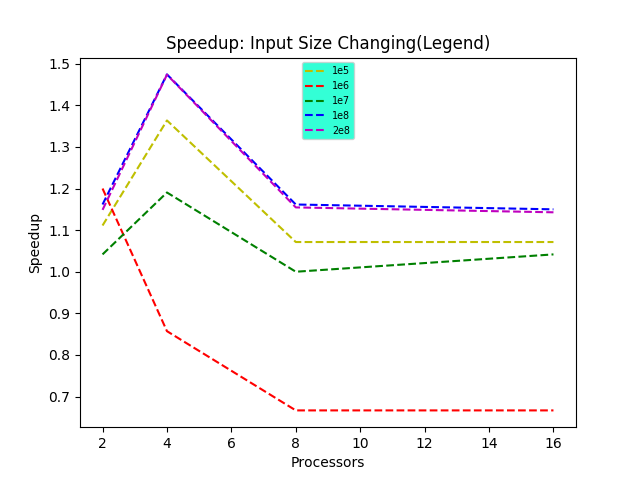
\includegraphics[scale=0.9]{Part1S.png}
\caption{Speedup vs Processors for Varying input}
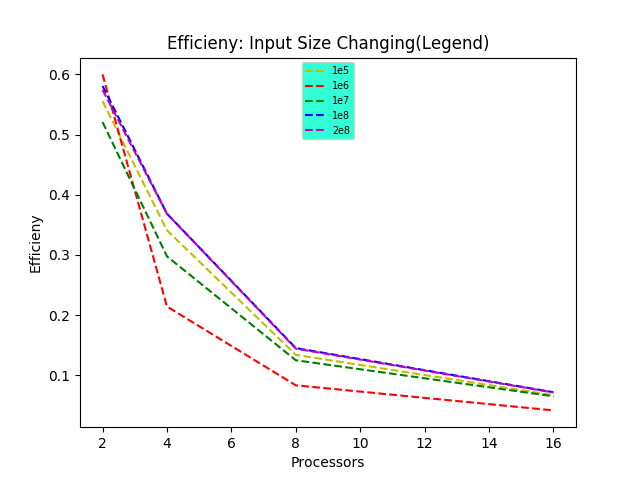
\includegraphics[scale=0.9]{Part1E.png}
\caption{Efficiency vs Processors for Varying input}
\end{figure}

\end{document}
